%----------------------------------------------------------------------------------------
%	PACKAGES AND THEMES
%----------------------------------------------------------------------------------------
\documentclass[aspectratio=169,xcolor=dvipsnames]{beamer}
\usetheme{SimplePlus}

\usepackage{hyperref}
\usepackage{graphicx} % Allows including images
\usepackage{booktabs} % Allows the use of \toprule, \midrule and \bottomrule in tables

%----------------------------------------------------------------------------------------
%	TITLE PAGE
%----------------------------------------------------------------------------------------

\title[short title]{ECHO Slides} % The short title appears at the bottom of every slide, the full title is only on the title page
\subtitle{These figures are in-process}

\author[Bonham] {Kevin Bonham}

\institute[Wellesley College] % Your institution as it will appear on the bottom of every slide, may be shorthand to save space
{
    Department of Biological Sciences \\
    Wellesley College
}
\date{\today} % Date, can be changed to a custom date


%----------------------------------------------------------------------------------------
%	PRESENTATION SLIDES
%----------------------------------------------------------------------------------------

\begin{document}

\begin{frame}
    % Print the title page as the first slide
    \titlepage
\end{frame}

\begin{frame}{Overview}
    % Throughout your presentation, if you choose to use \section{} and \subsection{} commands, these will automatically be printed on this slide as an overview of your presentation
    \tableofcontents
\end{frame}


%------------------------------------------------
\section{Demographics}
%------------------------------------------------

% -----------------------------------------------------------------------------

\begin{frame}{Demographics - Pi charts}
    \begin{columns}[c] % The "c" option specifies centered vertical alignment while the "t" option is used for top vertical alignment

        \column{.5\textwidth} % Right column and width
    
        \begin{figure}
        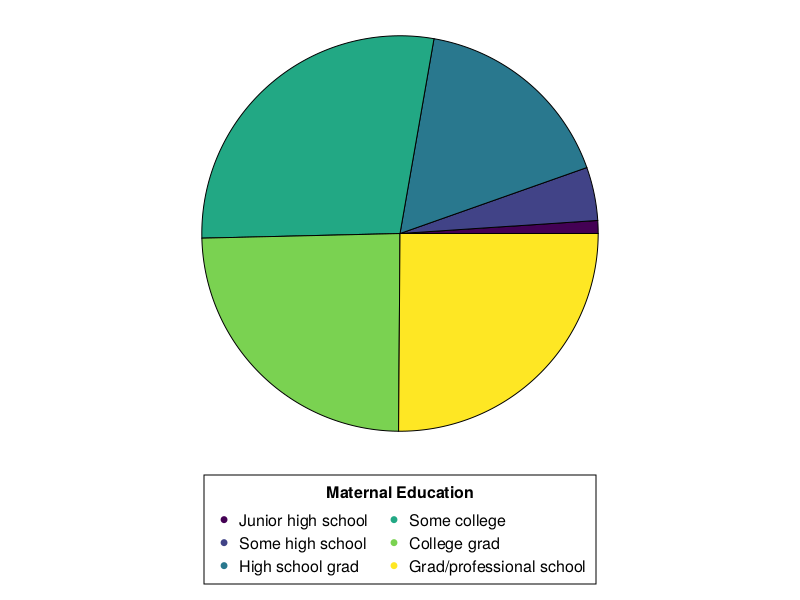
\includegraphics[width=1\linewidth]{../figures/demo_education.png}
        \end{figure}

        \column{.5\textwidth} % Right column and width
    
        \begin{figure}
        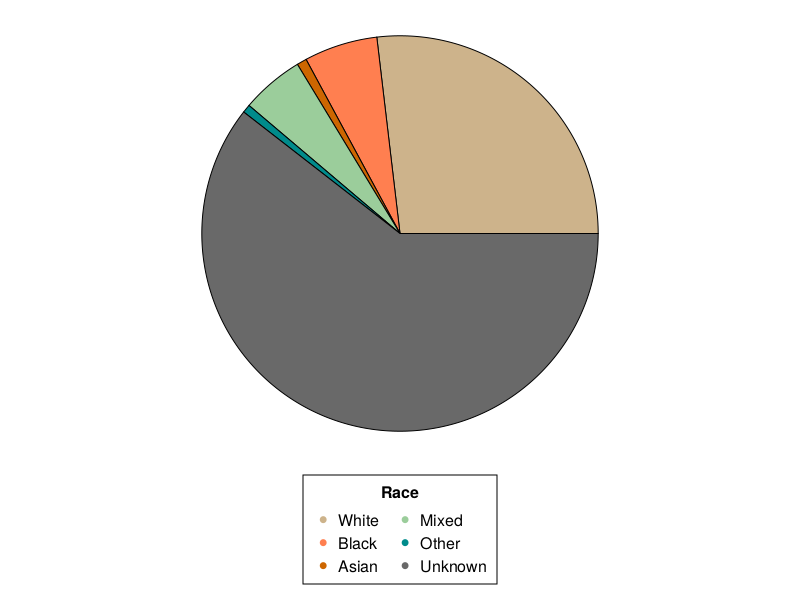
\includegraphics[width=1\linewidth]{../figures/demo_race.png}
        \end{figure}

    \end{columns}

    \textbf{Details}
    \begin{enumerate}
        \item Education does not include missings
        \item Race numbers not from database, using counts from RI group
    \end{enumerate}

\end{frame}

% -----------------------------------------------------------------------------



%------------------------------------------------
\section{Sample details}
%------------------------------------------------

% -----------------------------------------------------------------------------

\begin{frame}{Mother-child dyads}
    \begin{columns}[c] % The "c" option specifies centered vertical alignment while the "t" option is used for top vertical alignment

        \column{.6\textwidth} % Right column and width
    
        \begin{figure}
        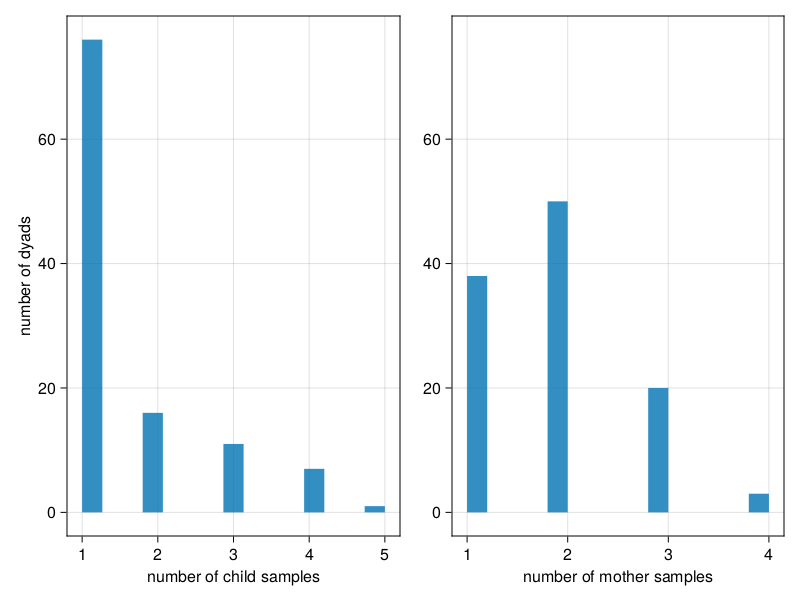
\includegraphics[width=1\linewidth]{../figures/dyads}
        \end{figure}

        \column{.4\textwidth} % Right column and width
    
        \textbf{Details}
        \begin{itemize}
            \item \textbf{Left} - Child samples that have at least 1 associated maternal sample
            \item \textbf{Right} - Maternal samples that have at least 1 associated child sample
        \end{itemize}

    \end{columns}

\end{frame}

% -----------------------------------------------------------------------------

\begin{frame}{Sample collection by age}
    \begin{columns}[c] % The "c" option specifies centered vertical alignment while the "t" option is used for top vertical alignment

        \column{.6\textwidth} % Right column and width
    
        \begin{figure}
        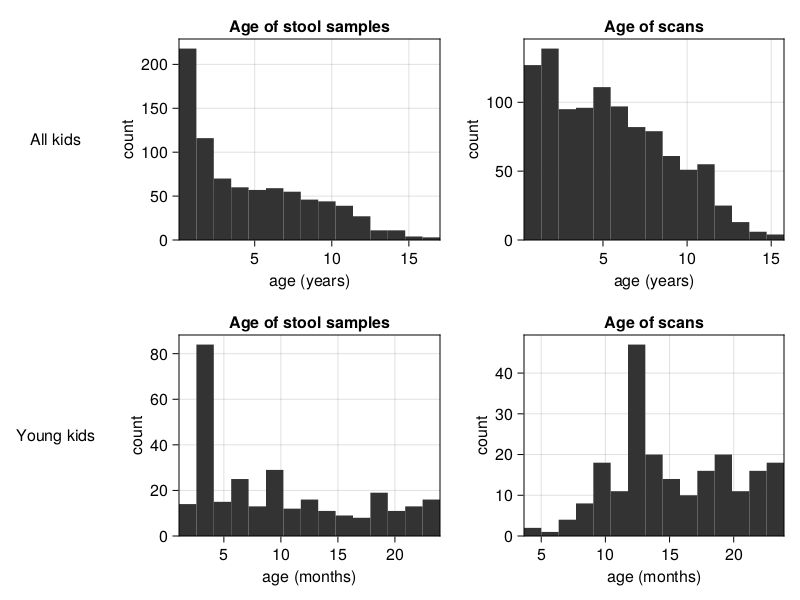
\includegraphics[width=1\linewidth]{../figures/age_hists}
        \end{figure}

        \column{.4\textwidth} % Right column and width
    
        \textbf{Details}
        \begin{itemize}
            \item Bottom row is same as top, but only from timepoints $<$ 24 months
        \end{itemize}

    \end{columns}

\end{frame}

% -----------------------------------------------------------------------------

\begin{frame}{Sample collection over time}
    \begin{columns}[c] % The "c" option specifies centered vertical alignment while the "t" option is used for top vertical alignment

        \column{.6\textwidth} % Right column and width
    
        \begin{figure}
        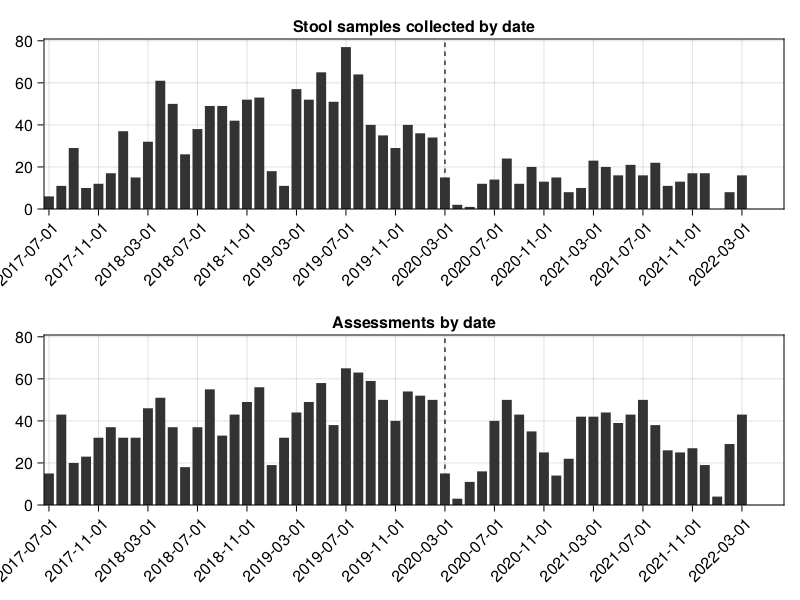
\includegraphics[width=1\linewidth]{../figures/collection_over_time}
        \end{figure}

        \column{.4\textwidth} % Right column and width
    
        \textbf{Details}
        \begin{itemize}
            \item \textbf{Top} - Stool samples (just omni) collected by date
            \item \textbf{Bottom} - Assessments (clinical visits) by date
        \end{itemize}

    \end{columns}

\end{frame}

% -----------------------------------------------------------------------------

\begin{frame}{Sample QC}
    \begin{columns}[c] % The "c" option specifies centered vertical alignment while the "t" option is used for top vertical alignment

        \column{.6\textwidth} % Right column and width
    
        \begin{figure}
        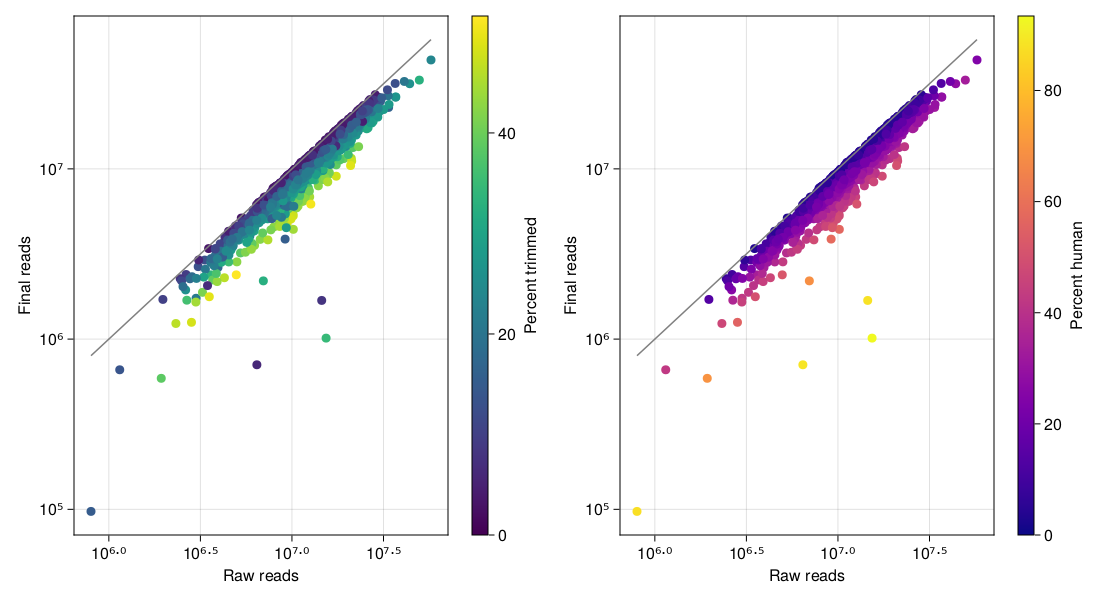
\includegraphics[width=1\linewidth]{../figures/kneaddata_counts}
        \end{figure}

        \column{.4\textwidth} % Right column and width
    
        \textbf{Details}
        \begin{itemize}
            \item Raw reads (x-axis) vs final QC'd reads (y-axis) after $kneaddata$ QC
            \item \textbf{Left} - Shows percent trimmed
            \item \textbf{Right} - Shows percent human reads
        \end{itemize}

    \end{columns}

\end{frame}

% -----------------------------------------------------------------------------

\begin{frame}{Upset - Brain scans + stool}
    \begin{columns}[c] % The "c" option specifies centered vertical alignment while the "t" option is used for top vertical alignment

        \column{.6\textwidth} % Right column and width
    
        \begin{figure}
        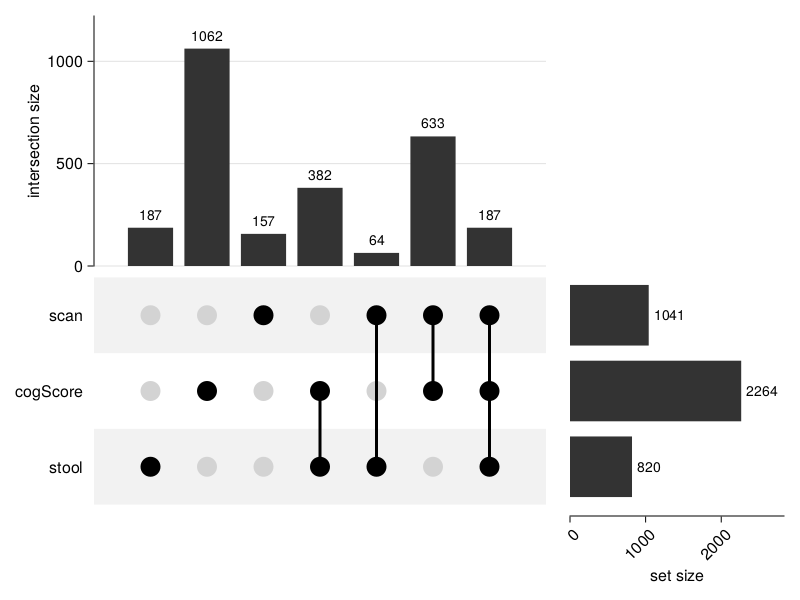
\includegraphics[width=1\linewidth]{../figures/upset_scan_stool.pdf}
        \end{figure}

        \column{.4\textwidth} % Right column and width
    
        \textbf{Details}
        \begin{itemize}
            \item Overlap of sample collection and brain scans
            \item "Prev stool" means that there's stool sample collected prior to timepoint
            \item Not 100\% sure of this code - needs review
        \end{itemize}

    \end{columns}

\end{frame}

% -----------------------------------------------------------------------------

\begin{frame}{Upset - By subject}
    \begin{columns}[c] % The "c" option specifies centered vertical alignment while the "t" option is used for top vertical alignment

        \column{.6\textwidth} % Right column and width
    
        \begin{figure}
        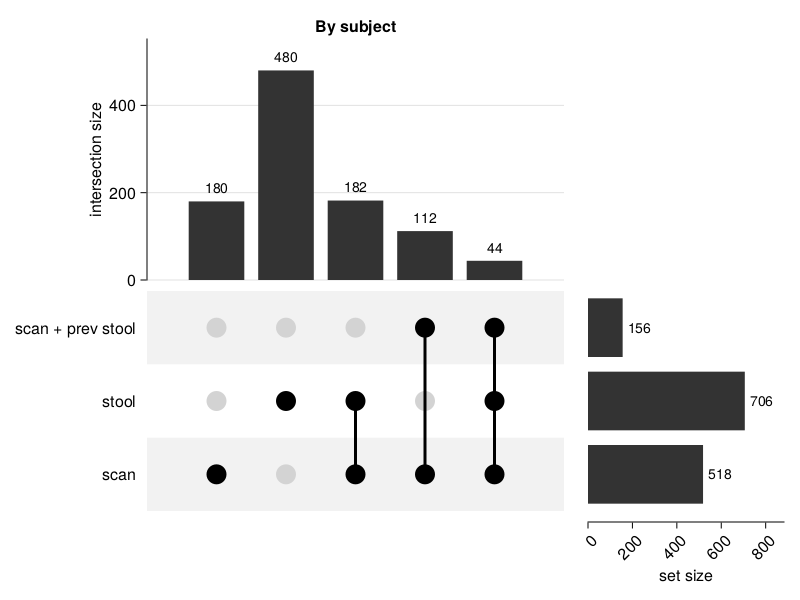
\includegraphics[width=1\linewidth]{../figures/upset_scan_stool_bysybject.pdf}
        \end{figure}

        \column{.4\textwidth} % Right column and width
    
        \textbf{Details}
        \begin{itemize}
            \item Overlap of sample collection and brain scans
            \item Numbers reduced to unique subjects
        \end{itemize}

    \end{columns}

\end{frame}

% -----------------------------------------------------------------------------

\begin{frame}{Upset - Overlaps with cogscore}
    \begin{columns}[c] % The "c" option specifies centered vertical alignment while the "t" option is used for top vertical alignment

        \column{.6\textwidth} % Right column and width
    
        \begin{figure}
        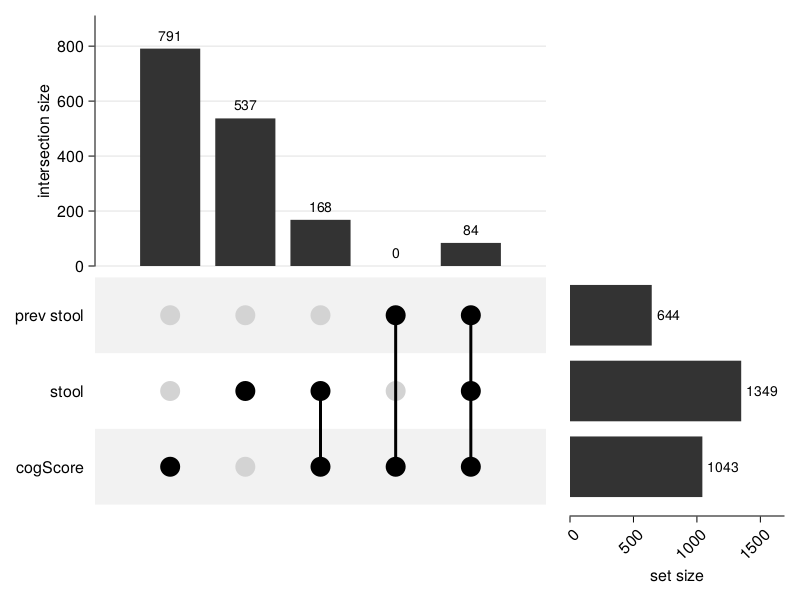
\includegraphics[width=1\linewidth]{../figures/upset_score_stool.pdf}
        \end{figure}

        \column{.4\textwidth} % Right column and width
    
        \textbf{Details}
        \begin{itemize}
            \item Overlap of sample collection and cognitive score
        \end{itemize}

    \end{columns}

\end{frame}

% -----------------------------------------------------------------------------
\begin{frame}{Upset - Kids under 3}
    \begin{columns}[c] % The "c" option specifies centered vertical alignment while the "t" option is used for top vertical alignment

        \column{.6\textwidth} % Right column and width
    
        \begin{figure}
        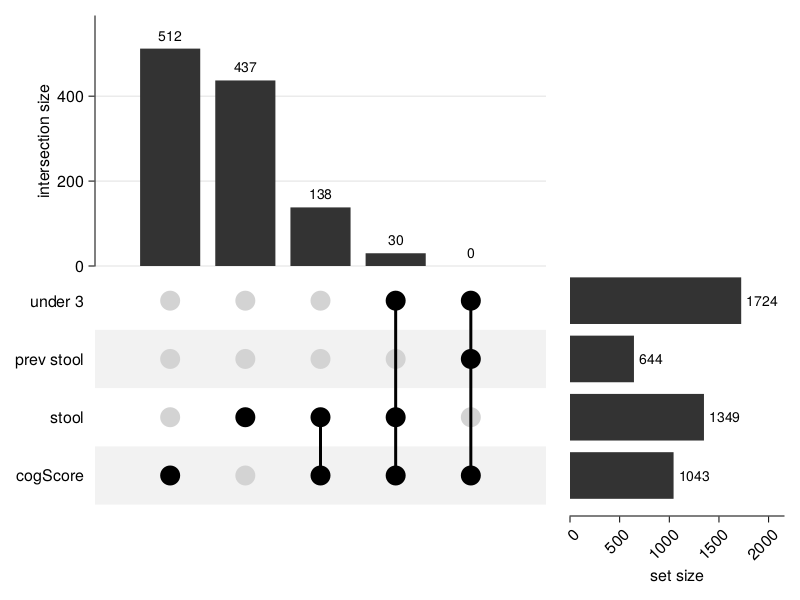
\includegraphics[width=1\linewidth]{../figures/upset_score_stool_under3.pdf}
        \end{figure}

        \column{.4\textwidth} % Right column and width
    
        \textbf{Details}
        \begin{itemize}
            \item Overlap of sample collection and cognitive score for kids under 3
            \item "Under 3" row is all timepoints, regardless of stool collection
        \end{itemize}

    \end{columns}

\end{frame}

% -----------------------------------------------------------------------------
\begin{frame}{Upset - By subject}
    \begin{columns}[c] % The "c" option specifies centered vertical alignment while the "t" option is used for top vertical alignment

        \column{.6\textwidth} % Right column and width
    
        \begin{figure}
        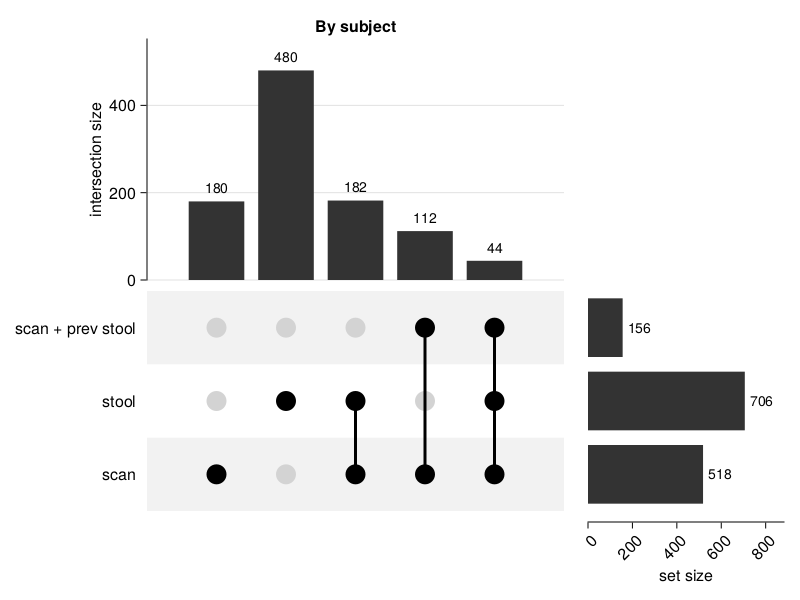
\includegraphics[width=1\linewidth]{../figures/upset_scan_stool_bysybject.pdf}
        \end{figure}

        \column{.4\textwidth} % Right column and width
    
        \textbf{Details}
        \begin{itemize}
            \item Numbers reduced to unique subjects
        \end{itemize}

    \end{columns}

\end{frame}

% -----------------------------------------------------------------------------


%------------------------------------------------
\section{Brain stuff}
%------------------------------------------------

% -----------------------------------------------------------------------------

\begin{frame}{Brain PCoA}
    \begin{columns}[c] % The "c" option specifies centered vertical alignment while the "t" option is used for top vertical alignment

        \column{.45\textwidth} % Left column and width
        \textbf{Details}
        \begin{enumerate}
            \item PCA, Euclidean distance of brain regions, normalized by total brain size
            \item All kids with processed brain scans
            \item Top: colored by age, first 2 axes
            \item Bottom: PCA1 x Age, colored by cogscore
            
        \end{enumerate}

        \column{.5\textwidth} % Right column and width
    
        \begin{figure}
        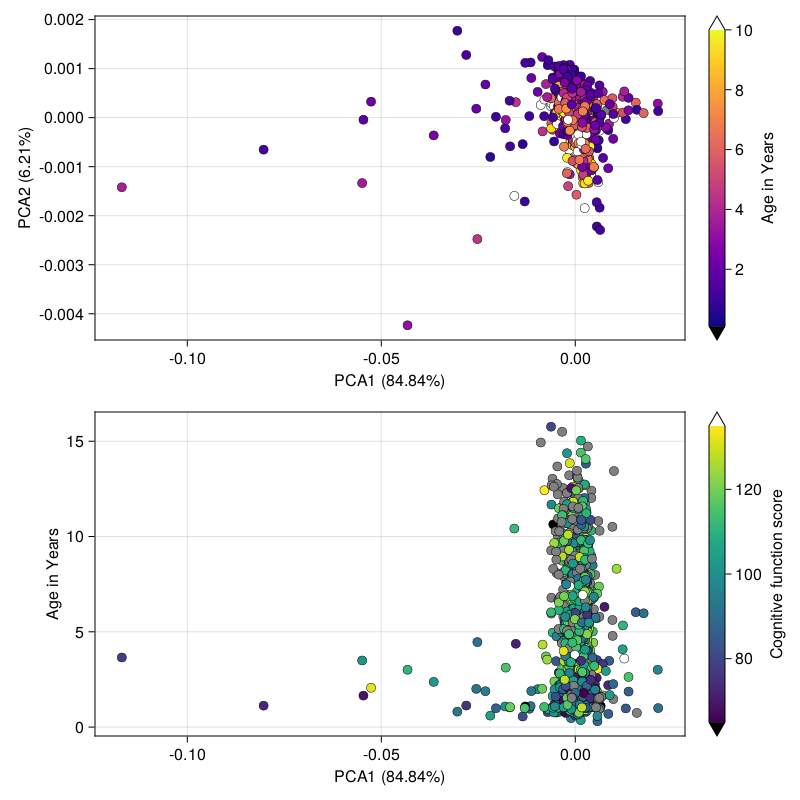
\includegraphics[width=1\linewidth]{../figures/brain_pcoa.png}
        \end{figure}

    \end{columns}
\end{frame}

% -----------------------------------------------------------------------------

\begin{frame}{Cognitive score summaries}
    \begin{columns}[c] % The "c" option specifies centered vertical alignment while the "t" option is used for top vertical alignment

        \column{.45\textwidth} % Left column and width
        
        \begin{figure}
            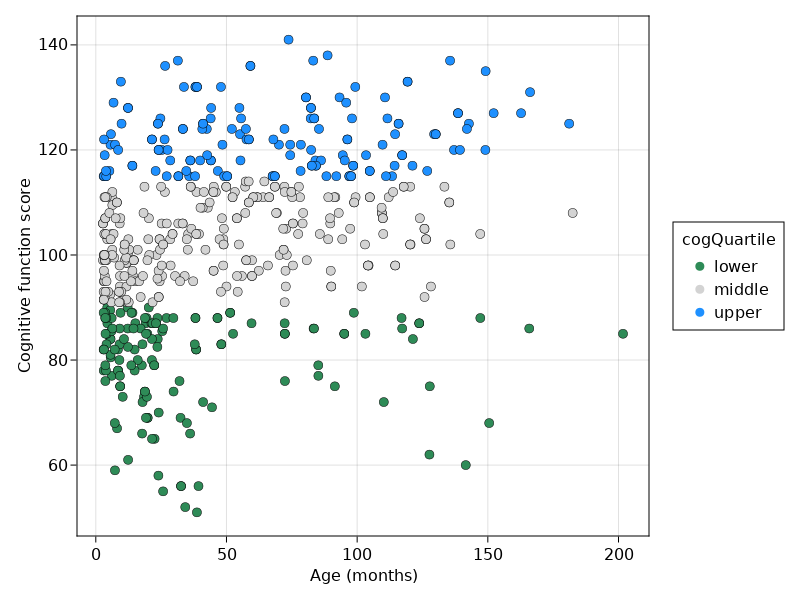
\includegraphics[width=1\linewidth]{../figures/cogScore_quartiles.png}
        \end{figure}

        \column{.5\textwidth} % Right column and width
    
        \begin{figure}
        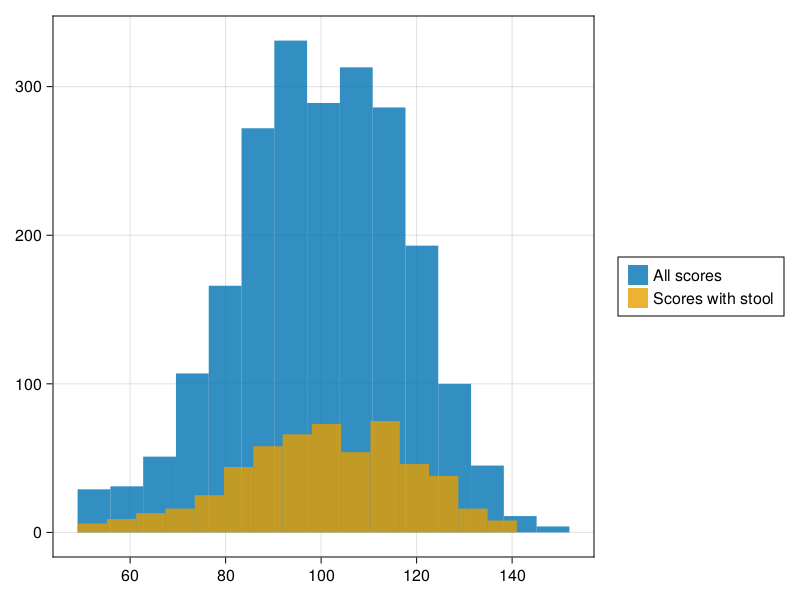
\includegraphics[width=1\linewidth]{../figures/cogscores_hist.pdf}
        \end{figure}

    \end{columns}

    \textbf{Details}
    \begin{enumerate}
        \item Quartiles calculated based on all measurements
    \end{enumerate}

\end{frame}

% -----------------------------------------------------------------------------


%------------------------------------------------
\section{Metabolits}
%------------------------------------------------

% -----------------------------------------------------------------------------

\begin{frame}{GABA and Glutamate}
    \begin{columns}[c] % The "c" option specifies centered vertical alignment while the "t" option is used for top vertical alignment

        \column{.5\textwidth} % Right column and width
    
        \begin{figure}
        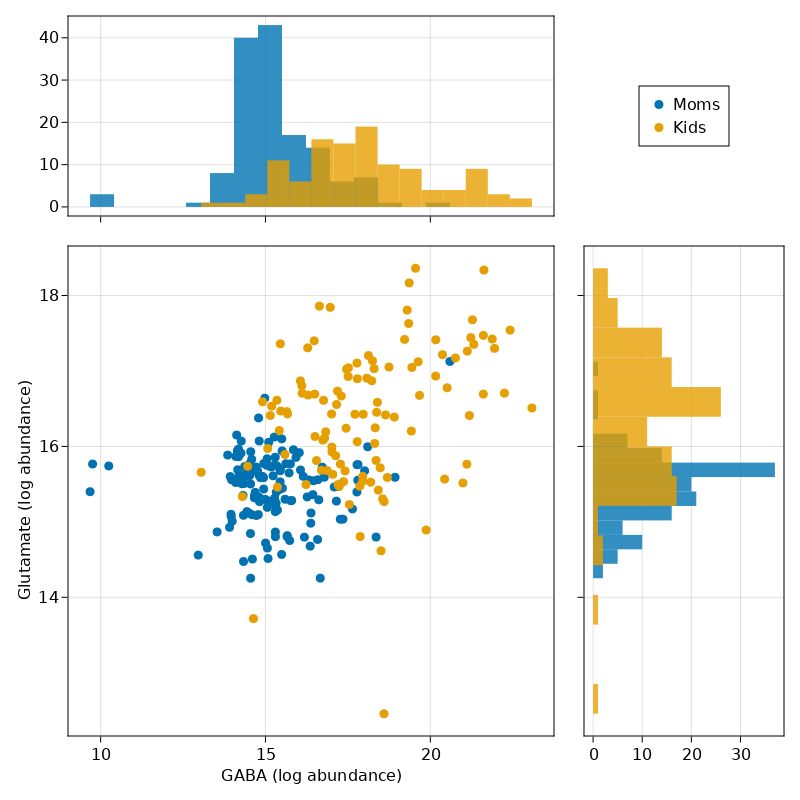
\includegraphics[width=1\linewidth]{../figures/gaba-glutamate.png}
        \end{figure}

        \column{.4\textwidth} % Right column and width
    
        \textbf{Details}
        \begin{itemize}
            \item Comparing mother and child samples
            \item Mean-centered and compositional
            \item Plotting $log_2(relative\_abundance)$
        \end{itemize}

    \end{columns}

\end{frame}

% -----------------------------------------------------------------------------

\begin{frame}{GABA and Glutamate, by age}
    \begin{columns}[c] % The "c" option specifies centered vertical alignment while the "t" option is used for top vertical alignment

        \column{.5\textwidth} % Right column and width
    
        \begin{figure}
        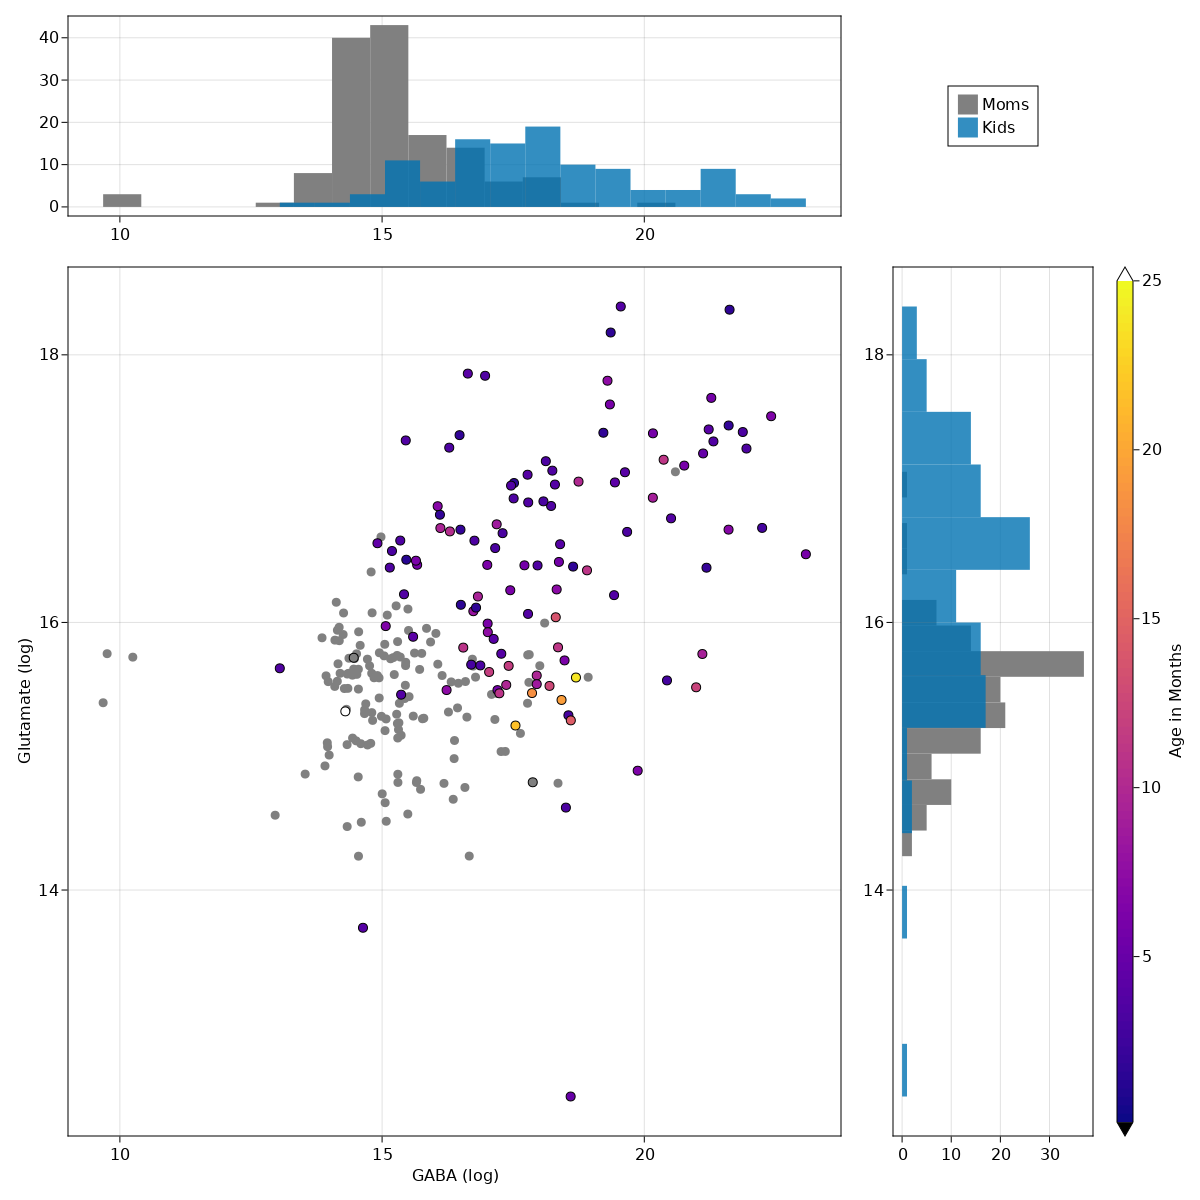
\includegraphics[width=1\linewidth]{../figures/gaba-glutamate_age.png}
        \end{figure}

        \column{.4\textwidth} % Right column and width
    
        \textbf{Details}
        \begin{itemize}
            \item Comparing mother and child samples
            \item Age in months colored, moms are gray
            \item Plotting $log_2(relative\_abundance)$
        \end{itemize}

    \end{columns}

\end{frame}

% -----------------------------------------------------------------------------

\begin{frame}{Metabolites PCoA}
    \begin{columns}[c] % The "c" option specifies centered vertical alignment while the "t" option is used for top vertical alignment

        \column{.5\textwidth} % Right column and width
    
        \begin{figure}
        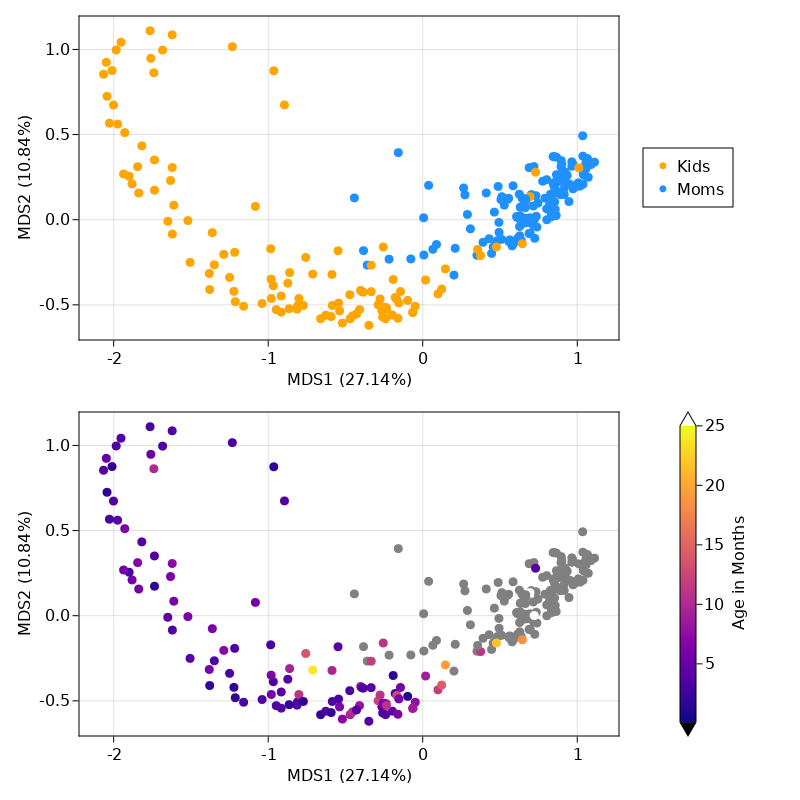
\includegraphics[width=1\linewidth]{../figures/metabolites_pcoa.png}
        \end{figure}

        \column{.4\textwidth} % Right column and width
    
        \textbf{Details}
        \begin{itemize}
            \item PCoA based on BC dissimilartiy
        \end{itemize}

    \end{columns}

\end{frame}

% -----------------------------------------------------------------------------


%------------------------------------------------
\section{Linear Models}
%------------------------------------------------

\begin{frame}{PERMANOVAs - all kids}
    \begin{columns}[c] % The "c" option specifies centered vertical alignment while the "t" option is used for top vertical alignment

        \column{.6\textwidth} % Right column and width
    
        \begin{figure}
        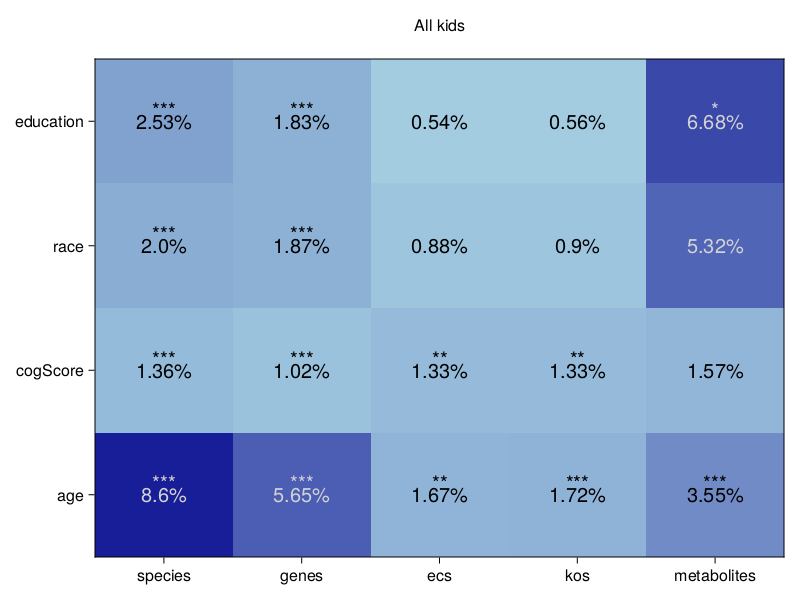
\includegraphics[width=1\linewidth]{../figures/kids_all_permanovas.png}
        \end{figure}

        \column{.4\textwidth} % Right column and width
    
        \textbf{Details}
        \begin{itemize}
            \item Single sample (first) per kid
            \item Univariate permanova
            \item For KOs / ECs, UNGROUPED features were excluded, UNMAPPED were included
        \end{itemize}

    \end{columns}

\end{frame} 

\begin{frame}{PERMANOVAs - kids under 6 months old}
    \begin{columns}[c] % The "c" option specifies centered vertical alignment while the "t" option is used for top vertical alignment

        \column{.6\textwidth} % Right column and width
    
        \begin{figure}
        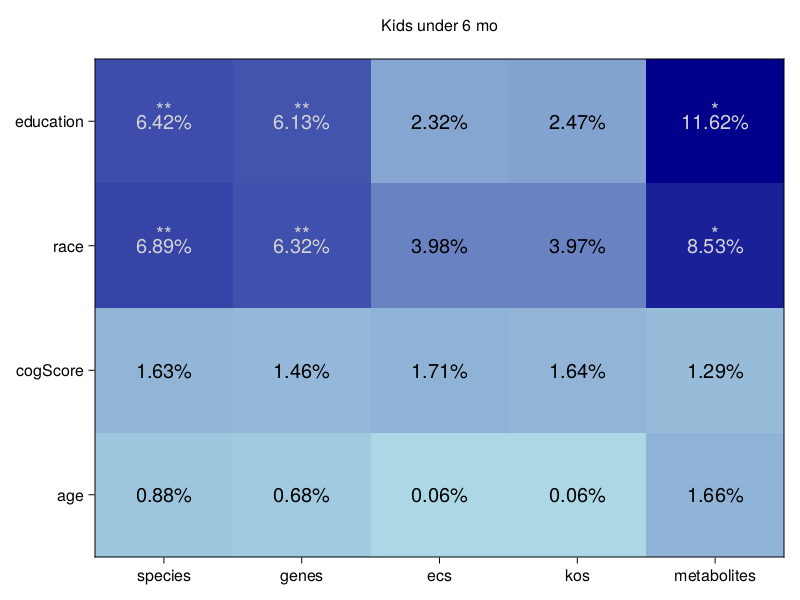
\includegraphics[width=1\linewidth]{../figures/kids_under6mo_permanovas.png}
        \end{figure}

        \column{.4\textwidth} % Right column and width
    
        \textbf{Details}
        \begin{itemize}
            \item Single sample per kid
            \item Univariate permanova
            \item For KOs / ECs, UNGROUPED features were excluded, UNMAPPED were included
        \end{itemize}

    \end{columns}

\end{frame}

\begin{frame}{PERMANOVAs - kids over 1 year old}
    \begin{columns}[c] % The "c" option specifies centered vertical alignment while the "t" option is used for top vertical alignment

        \column{.6\textwidth} % Right column and width
    
        \begin{figure}
        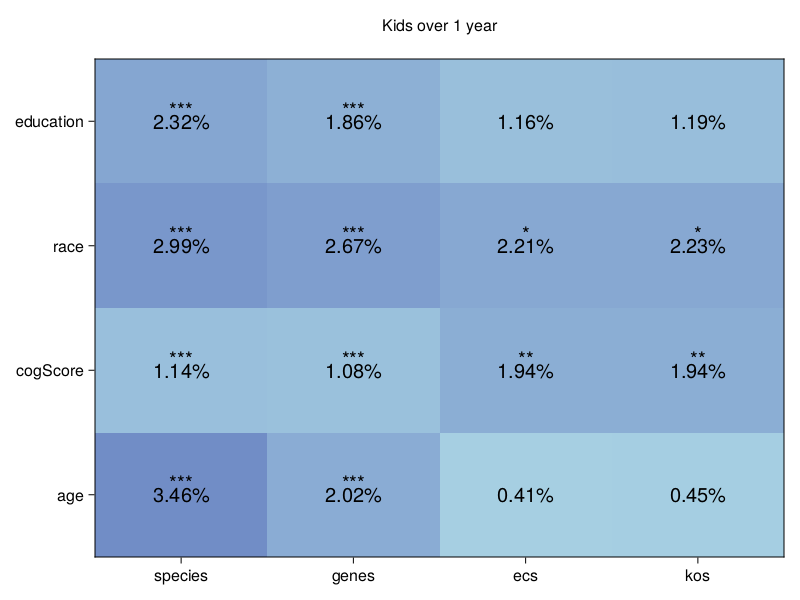
\includegraphics[width=1\linewidth]{../figures/kids_over1y_permanovas.png}
        \end{figure}

        \column{.4\textwidth} % Right column and width
    
        \textbf{Details}
        \begin{itemize}
            \item Single sample per kid
            \item Univariate permanova
            \item For KOs / ECs, UNGROUPED features were excluded, UNMAPPED were included
            \item Metabolites not included because there are only a few samples over 1 year
        \end{itemize}

    \end{columns}

\end{frame}


\begin{frame}{Mantel tests}
    \begin{columns}[c] % The "c" option specifies centered vertical alignment while the "t" option is used for top vertical alignment

        \column{.6\textwidth} % Right column and width
    
        \begin{figure}
        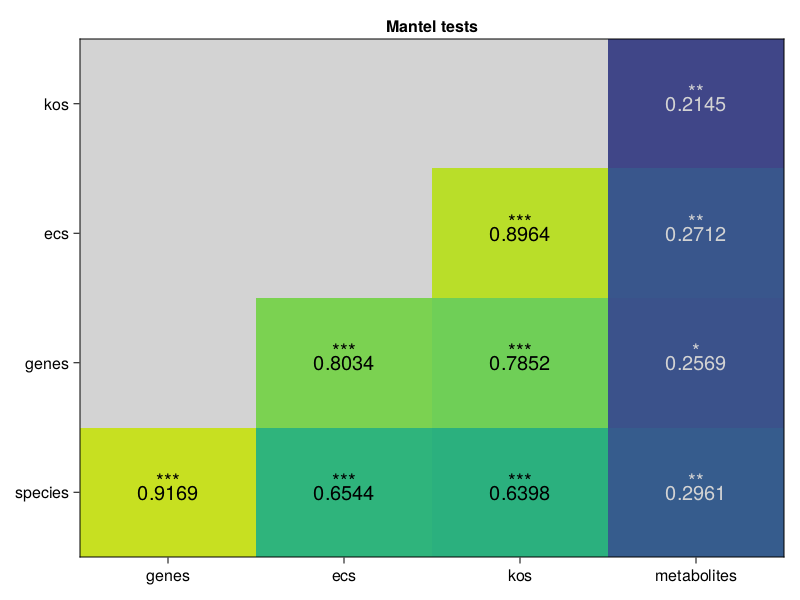
\includegraphics[width=1\linewidth]{../figures/mantel.png}
        \end{figure}

        \column{.4\textwidth} % Right column and width
    
        \textbf{Details}
        \begin{itemize}
            \item Run on all kids - one sample per kid
            \item Mantel test asks how much of the variation across datasets is similar
        \end{itemize}

    \end{columns}

\end{frame}

\begin{frame}{Linear models - taxa}
    \begin{columns}[c] % The "c" option specifies centered vertical alignment while the "t" option is used for top vertical alignment

        \column{.6\textwidth} % Right column and width
    
        \begin{figure}
        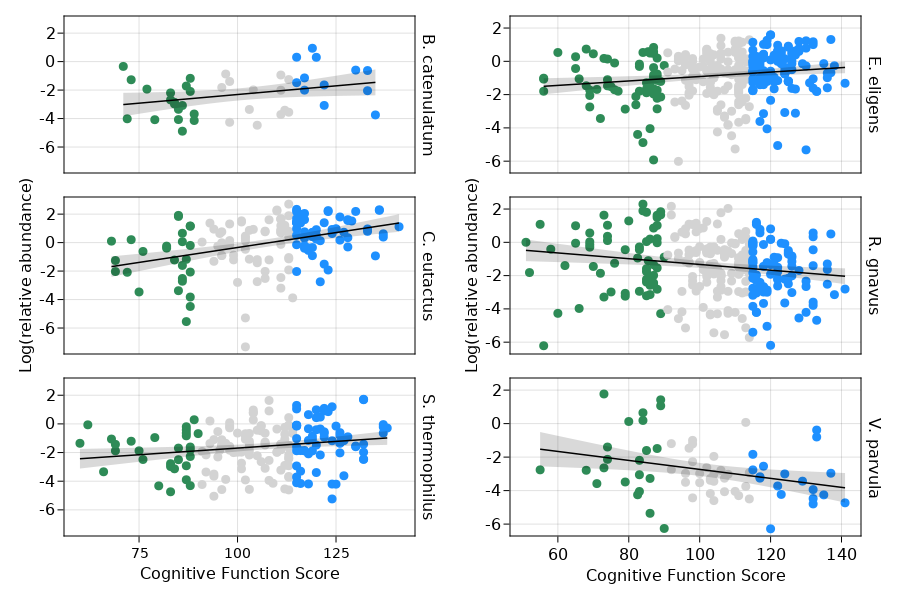
\includegraphics[width=1\linewidth]{../figures/lms-split-2.png}
        \end{figure}

        \column{.4\textwidth} % Right column and width
    
        \textbf{Details}
        \begin{itemize}
            \item Kids $> 18$ months old, species $> 10\%$ prevalence
            \item GLM: $bug \sim cogScore + age$
            \item There were ~15 bugs significant after FDR correction
        \end{itemize}

    \end{columns}

\end{frame}


\begin{frame}
    \Huge{\centerline{\textbf{The End}}}
\end{frame}

%----------------------------------------------------------------------------------------

\end{document}